%%%%%%%%%%%%%%%%%%%%%%%%%%%%%%%%%%%%%%%%%%%%%%%%%%%%%%%%%%%%%%%%%%%%%%%%%%%%
%% Trim Size : 11in x 8.5in
%% Text Area : 9.6in (include Runningheads) x 7in
%% ws-jai.tex, 26 April 2012
%% Tex file to use with ws-jai.cls written in Latex2E.
%% The content, structure, format and layout of this style file is the
%% property of World Scientific Publishing Co. Pte. Ltd.
%%%%%%%%%%%%%%%%%%%%%%%%%%%%%%%%%%%%%%%%%%%%%%%%%%%%%%%%%%%%%%%%%%%%%%%%%%%%
%%

%\documentclass[draft]{ws-jai}
\documentclass{ws-jai}
\usepackage[flushleft]{threeparttable}
\usepackage{pdflscape}
\usepackage{longtable}
\def\btex{B{\sc IB}\TeX\ }
\begin{document}

\catchline{}{}{}{}{} % Publisher's Area please ignore

\markboth{Jack Hickish, CASPER gang, etc.}{The Collaboration for Astronomy Signal Processing and Electronics Research in 2016.}

\title{The Collaboration for Astronomy Signal Processing and Electronics Research in 2016}

%\author{First Author$^\dagger$, Second Author$^\ddagger$, Third Author$^\ddagger$ and Fourth Author$^\S$}
\author{Jack Hickish$^\dagger$, Others$^\ddagger$}

\address{
$^\dagger$Radio Astronomy Laboratory, UC Berkeley, Berkeley, CA 94720, USA, jackh@astro.berkeley.edu\\
$^\ddagger$Group, Company, Address, City, State ZIP/Zone, Country\\
$^\S$Group, Company, Address, City, State ZIP/Zone, Country, fauthor@company.com
}

\maketitle

\corres{$^\dagger$Jack Hickish}

\begin{history}
\received{(to be inserted by publisher)};
\revised{(to be inserted by publisher)};
\accepted{(to be inserted by publisher)};
\end{history}

\begin{abstract}

The Collaboration for Astronomy Signal Processing and Electronics Research
(CASPER) has been working for a decade to reduce the time and cost of designing,
building and deploying new digital radio astronomy instruments.  Today,
CASPER-designed hardware powers over 40 scientific instruments worldwide, and
are used by scientists and engineers at dozens of academic institutions.  In this paper
we summarize the current offerings of the CASPER collaboration, focusing on
currently-available and next-generation hardware.  We describe the ongoing state
of software development, as CASPER looks to support an ever-increasing selection
of off-the-shelf digital signal processing platforms.

\end{abstract}

\keywords{CASPER, digital signal processing, radio astronomy, instrumentation}

\section{Introduction}

Since the first digital instrument used in radio astronomy \citep{Weinreb} we
have seen a growing adoption of digital processing hardware as the foundation on
which radio telescopes are built.  Today, CPUs, GPUs, FPGAs and ASICs power
almost all of the world's radio telescopes, and our ability to do science has
become inextricably linked with our ability to perform digital computation.
With the capability of digital processing hardware scaling exponentially with
Moore's law, the ability to leverage current technology by reducing the
design-time of new instruments is critical in effective deployments of new radio
astronomy instruments.

The Collaboration for Astronomy Signal Processing and Electronics Research
(CASPER) puts \emph{time-to-science}, the time between conception of an
instrument and its deployment, as a central figure of merit in instrument
design. CASPER works to minimize time-to-science by working to develop and
support open-source, general-purpose hardware, software libraries and
programming tools which allow rapid instrument design, and straightforward
upgrade cycles.

With CASPER hardware and software now powering over 40 radio astronomy
instruments worldwide (see Tables~\ref{table:casper-instruments-spectrometers}, \ref{table:casper-instruments-mkids}, \ref{table:casper-instruments-correlators}) including some
of the largest, most advanced telescopes ever built, such as the upcoming
MeerKat Array\footnote{\url{http://public.ska.ac.za/meerkat/meerkat-schedule}}, the newly commissioned Five-hundred metre Spherical Aperture Telescope (FAST, \cite{fast}), and the Robert C. Byrd Green Bank Telescope \citep{vegas}, it is appropriate to document the state of the
Collaboration.

In this paper, we first summarize the design philosophy of CASPER in
Section~\ref{sec:CASPER-philosophy}.  In Section~\ref{sec:Hardware} we describe
currently available CASPER hardware offerings, including the range of digitizers
developed and supported by CASPER. Key to CASPER's success are the firmware
libraries and programming infrastructure provided by the collaboration, which we
overview in Section~\ref{sec:Software}.  In Section~\ref{sec:Deployments} we
document the extensive and wide-ranging applications to which CASPER hardware
and design-tools have been applied. Finally, we describe the future direction of
and challenges faced by the CASPER collaboration in Section~\ref{sec:Future},
with concluding remarks in Section~\ref{sec:Conclusions}.

\section{The CASPER Philosophy} \label{sec:CASPER-philosophy}

%% Jason Manley's PHD has a good section on Philosophy and Ethernet.


World-wide, radio astronomy is a relatively small industry and has minimal financial incentive attracting investors. This means that often institutions often rely heavily on government funding. It is therefore beneficial to share resources between organisations as to leverage the work that others have put into developing radio astronomy instrumentation. For this reason institutions often open source their intellectual property. CASPER was founded to aid this collaboration. It aims to share and collaborate on both hardware and software for the design of radio astronomy DSP systems.

The CASPER community has designed multiple FPGA based hardware platforms and the software tools to design and support these platforms.

Along with hardware platforms, CASPER provides a tool-flow based on the Matlab, Simulink and Xilinx System Generator (XSG) tools to enable a designer to easily design and target a particular hardware platform \cite{pars05}. The interface is a graphical design environment in Simulink where a designer can drag and drop blocks and connect them with wires in the desired configuration. A library of CASPER Digital Signal Processing (DSP) blocks are provided. These are targeted at the particular type of DSP typical of radio astronomy data processing. In addition, there is also a library of hardware specific blocks, which contain the controllers for ADCs and Ten Gigabit Ethernet (TGE) modules, amongst others. The flow provides a "One-Click" solution from design to bitstream, ready to upload onto a board. The DSP parts of the design are easily transferable to other Xilinx FPGA hardware. This eases upgrades to new hardware, as well as aiding collaboration between teams using different CASPER hardware platforms \cite{pars05}.

CASPER makes use of Ethernet as a generic backplane architecture, to provide packetised interconnects between hardware modules. In this way, instruments can consist of different types of data processing hardware. For example, it is easy to hand off parts of the processing chain to a GPU cluster by redirecting the data sent over the network to different Internet Protocol (IP) address. A design can even leverage the IP Multicast protocol\footnote{IP multicast is described in RFC 1112} which allows additional instruments to subscribe to the data and process it concurrently alongside the main instrument. This keeps the problem of full cross-bar interconnects in the domain of the switch manufactures and allows instrument designers to focus on digital signal processing \cite{man14}, \cite{pars05}.

Overall, CASPER has a progressive philosophy towards instrumentation design and it is important to take into account when examining, designing and implementing tools to be used by this community and others.

\subsection{Computing by the yard}

\subsection{Ethernet}

\subsubsection{Multicast \& Commensal Instruments}


\section{CASPER Hardware} \label{sec:Hardware}

Since its inception, the collaboration has produced a range of hardware with particular focus on FPGA boards and supporting hardware such as Analog-to-Digital Converters (ADC) and Ethernet mezzanine cards.

\subsection{FPGA platforms}

Much of the focus of the community has moved from the popular ROACH2 platform to the newer SNAP and SKARAB boards which sport the Xilinx Kintex and Virtex FPGAs, respectively. This section, therefore, will focus on the SKARAB and SNAP hardware platforms.

\subsubsection{ROACH1}

For completeness it is important to mention the grandfather of the current hardware generation, the ROACH1. The architecture is based on a single FPGA with a control processor and mezzanine connectors for the addition of ADCs and other peripherals \cite{Casp09}. The core of the ROACH is the Xilinx Virtex 5 xc5vlx110t chip. The CASPER tools still provide support for this board even though it is two generations old.

%% Wesley New

\subsubsection{ROACH2}

The ROACH2 is the update to the ROACH platform, the major differences being the Xilinx Virtex 6 FPGA and the addition of two mezzanine slots which could be used for memory or Ethernet cards \cite{Casp12}.
%% Wesley New

\subsubsection{SKARAB}

The Square Kilometre Array Reconfigurable Application Board (SKARAB) hardware is the next generation FPGA hardware platform that has been designed by a South African company, Peralex, according to the specifications of SKA-SA, as an alternative to the ROACH2 hardware for applications requiring better processing performance. The departure from the ``ROACH'' naming convention to the ``SKARAB'' naming convention is because the interfaces between the ROACH2 and the SKARAB are not compatible.

A functional block diagram of the SKARAB is presented in Figure~\ref{fig:skarab_bd} \cite{cliff16}.

\begin{figure}[h]
\centering
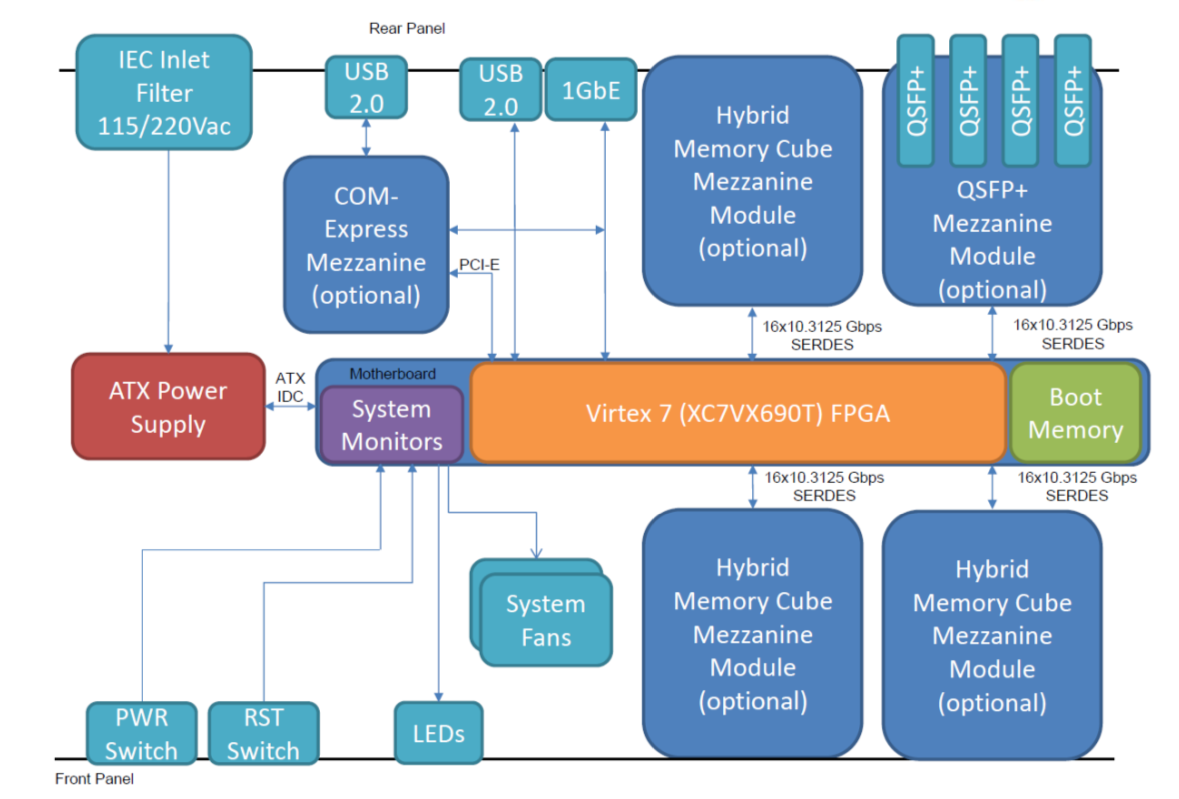
\includegraphics[width=150mm, scale=0.5]{skarab_bd}
\caption{SKARAB Functional Block Diagram}
\label{fig:skarab_bd}
\end{figure}

At the heart of the SKARAB processing, lies the Xilinx Virtex 7 FPGA (XC7VX690T). This FPGA consists of 693120 logic cells, 52 Mb of internal random access memory (RAM) blocks and 3600 digital signal processing (DSP) slices \cite{cliff16}. Nearly all of the input/output (I/O) available is high-speed serial/deserializer (SERDES) I/O \cite{Teag15}.

The SKARAB makes provision for four mezzanine sites with each site interfacing with sixteen transmit and sixteen receive 10 Gbps SERDES lines \cite{cliff16}. This means each site can handle a throughput of 160 Gbps and if all the sites are utilized, a total of 640 Gbps can be achieved.

There is no power personal computer (PPC), but provision has been made for the COM Express mezzanine site which can interface with an external processor via single lane PCIe \cite{Teag15}.

The SKARAB has already been tested with two existing mezzanine cards: QSFP+ Mezzanine Module and the Hybrid Memory Cube (HMC) Mezzanine Module. The Peralex QSFP+ Mezzanine Module supports four 40Gb Ethernet interfaces and the SKA-SA HMC Mezzanine module provides external memory storage for the processing using high speed serial memory \cite{cliff16}.

The hardware of the SKARAB is presented in Figure~\ref{fig:skarab_hw} \cite{cliff16}.

\begin{figure}[h]
\centering
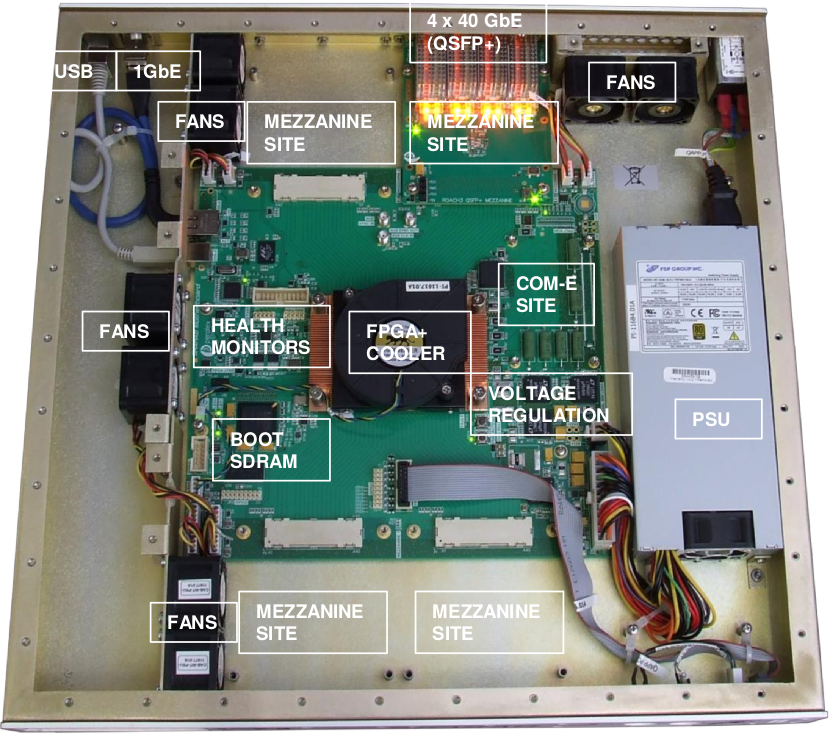
\includegraphics[width=150mm, scale=0.5]{skarab_hw}
\caption{SKARAB Hardware}
\label{fig:skarab_hw}
\end{figure}

The SKARAB board support package (BSP) comes with the 40GbE core, 1GbE core, HMC core and the management microcontroller, which runs on the FPGA (Xilinx's microblaze processor) \cite{cliff16}. The management microcontroller sets up the network (1GbE, 40GbE), performs FPGA configuration (1GbE), monitors the voltages and currents, monitors and controls the fan speeds and handles communication to/from the FPGA via the wishbone bus \cite{cliff16} \cite{Teagu15}.

The SKARAB BSP is currently being added to the CASPER tool flow and should be ready in December 2016.
SKA-SA will be integrating 300 SKARAB units, as part of the MeerKAT upgrades, and should be ready for operation latest by the end of 2017.

%% Adam Isaacson

\subsubsection{SNAP}

%% Rachel Domagalski
The Smart Network ADC Processor (SNAP) hardware is a lightweight next generation
FPGA platform designed primarily as digitizing elements in the Hydrogen Epoch of
Reionization Array (HERA) experiment. The SNAP board comes with onboard ADC's, a
frequency synthesizer, two 10 Gbit Ethernet, and the FPGA on SNAP (the Kintex
XC7K160T-2FFG676C chip) uses low power consumption, making the SNAP board useful
for larger arrays. SNAP is a low-cost board. The SNAP board has one ZDOK
connector enabling the use of the ADC cards listed below, and SNAP's onboard
ADC's have the same specifications as the ADC16x250-8. The FPGA on the SNAP can
be clocked either with an external frequency oscillator or with the TI LMX2581
frequency synthesizer onboard the SNAP. The SNAP board comes with a 40-pin
ribbon connector to interface with a  Raspberry Pi or similar computer. The
interface to the Raspberry Pi enables the SNAP board to easily be used as a
standalone spectrometer. FPGA gateware for the SNAP is developed using the
JASPER tool-flow. The SNAP hardware is presented in Figure~\ref{fig:snap_hw}.

\begin{figure}[h]
\centering
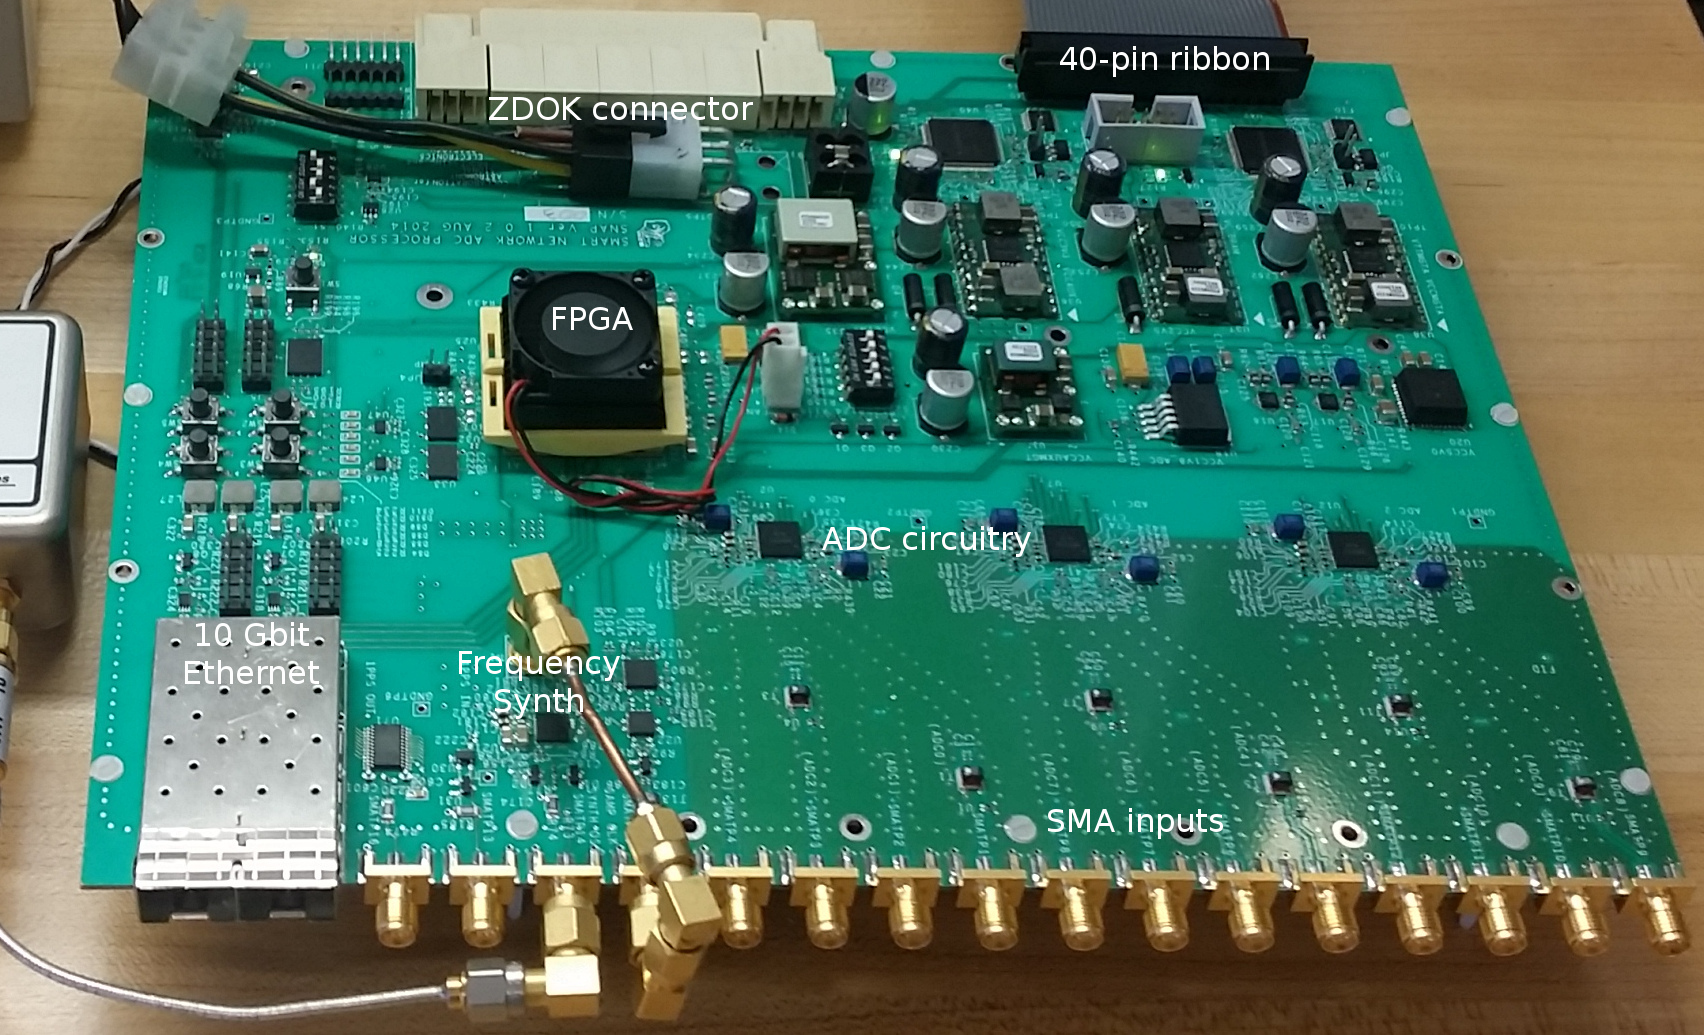
\includegraphics[width=150mm, scale=0.5]{snap_hw}
\caption{SNAP Hardware}
\label{fig:snap_hw}
\end{figure}

\subsection{ADCs \& DACs}

A number of high-speed, analogue interface boards have been developed to work
with the low-voltage, differential signaling (LVDS) Z-DOK interface, see Table
\ref{table:adcs_dacs}. The majority of these interface boards are analogue to
digital converters (ADCs) used to digitize the receiver signals. The extant ADCs
cover a broad range of instrument requirements typical in radio
astronomy. For example, the iADC is a two input, 8-bit dynamic range, 1000 Msps
digitiziter. The typical naming convention is ADC[number of inputs]x[sample
rate]-[bit width]. In addition to the ADCs a digital to analogue converter (DAC)
has been developed which has two 16-bit dynamic range, 1000 Msps outputs. For
each analogue interface board a `yellow block' is included in the DSP library,
see Section \ref{sec:dsp-libraries}.

% NOTE: I just took the list from the website, are there others, are these all legit? (Griffin)
\begin{tabular}{lccccc}
\label{table:adcs_dacs}
Name & Type & Bits & Sample Rate & Inputs/Outputs & Interface \\
\hline
ADC2x1000-8 (iADC) & ADC & 8 & 1 GSPS & 2 & Z-DOK \\
ADC1x3000-8 & ADC & 8 & 3 GSPS & 1 & Z-DOK \\
ADC64x64-12 & ADC & 12 & 64 MSPS & 64 & Z-DOK x2 \\
ADC4x250-8 (QuADC) & ADC & 8 & 250 MSPS & 4 & Z-DOK \\
ADC2x550-12 & ADC & 12 & 550 MSPS & 2 & Z-DOK \\
ADC2x400-14 & ADC & 14 & 400 MSPS & 2 & Z-DOK \\
KatADC & ADC & 8 & 1.5 GSPS/3.0 GSPS & 2/1 & Z-DOK \\
ADC1x5000-8 & ADC & 8 & 5 GSPS & 1 & Z-DOK \\
ADC16x250-8 & ADC & 8 & 1 GSPS/500 MSPS/250 MSPS & 4/8/16 & Z-DOK \\
ADC1x10000-4 & ADC & 4 & 10 GSPS & 1 & Z-DOK \\
DAC2x1000-16 & DAC & 16 & 1 GSPS & 2 & Z-DOK \\
\end{tabular}

\section{CASPER Software \& Programming Tools} \label{sec:Software}

\subsection{The CASPER Tool Flow}

%% Wesley New

\subsection{JASPER Tool Flow}

%% Jack Hickish to introduce this and explain history

%% Adam Isaacson to explain the latest additions
The JASPER tool flow is currently being upgraded to make provision for additional front ends and back ends besides Simulink and Xilinx, respectively. This will prevent the developer from being tied down to a specific software package and FPGA platform \cite{Isaac16}. The current upgrades are presented in Figure~\ref{fig:jasper_ug_bd} \cite{Isaac16}.

\begin{figure}[h]
\centering
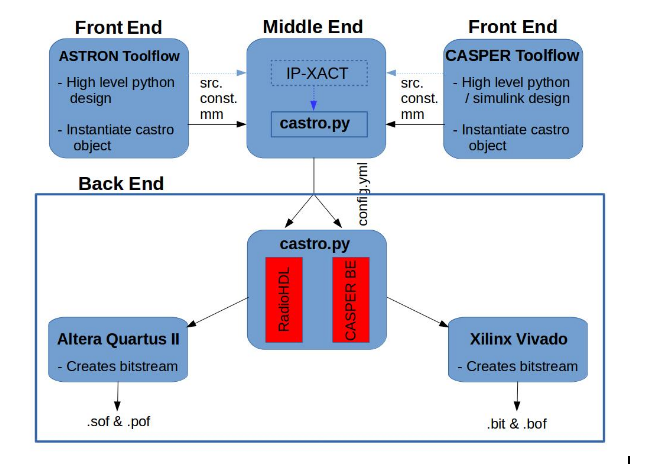
\includegraphics[width=150mm, scale=0.5]{jasper_ug_bd}
\caption{JASPER Upgrade Tool Flow Diagram}
\label{fig:jasper_ug_bd}
\end{figure}

The Front-End includes the structural VHDL or any modelling tools e.g. Matlab/Simulink, Labview, Sci-Lab/Sci-Cos and MyHDL. It includes a script which will instantiate the python classes inside the Middle End process \cite{Isaac16}.

The python classes are located in the Middle End (castro.py) file. In the future, it is likely that the Front End will come in through another interface e.g. possibly IP-XACT in order to make provision to interface to other simulation tools e.g. Sci-Cos and Sci-Lab. This interface is denoted by the dashed lines in Figure~\ref{fig:jasper_ug_bd}. IP-XACT is an IEEE standard and is used to integrate different IP packages together, provided that the IP interfacing meets the IP-XACT standard. The IP-XACT interface would be in the form of an XML script. The decision to utilise IP-XACT has not been finalised yet. The castro.py is passed all the Front End memory map, constraints and source files. The castro.py script takes this metadata from the Front End and dumps all of this metadata into a YAML configuration file (config.yml). It should be noted that the Middle End module is not platform agnostic due to the hardware and platform metadata \cite{Isaac16}.

The Back End consists of the same castro python class that exists in the Middle End. The castro.py python script will load the config.yml file/metadata and instantiate python objects with this metadata, which will either be sent to RadioHDL if targeting the Altera hardware or the Casper Back End, if targeting the Xilinx hardware. This will also allow the user to target other vendor hardware in the future e.g. Lattice and Actel and due to the common castro.py python script, it will easier to just add an additional back end \cite{Isaac16}.

The RadioHDL process will then generate the necessary Quartus project files and run the compiler. The output of the process will be the Altera FPGA SRAM Object file (sof) and Programming Object File (pof). The Casper Back End generates the necessary tcl scripts, which runs the Vivado compiler. The output of the process is the Xilinx FPGA bit and Borph Object File (bof) programmable files \cite{Isaac16}.

The current release of the JASPER tool flow actually includes the castro python class and the CASPER back end makes provision for both Xilinx ISE and Vivado. The JASPER tool flow also makes provision for the SKARAB platform and the generation of the fpg configuration files, which are used for the ROACH2 and SKARAB configuration \cite{Balla16}.

%% Adam Isaacson / Jack Hickish

\subsection{CASPER DSP Libraries}
\label{sec:dsp-libraries}

%% Andrew Martens + anyone else keen to contribute

% NOTE: First draft of section, please feel free to edit (Griffin)

In order to quickly and easily develop new radio astronomy instruments a number
of DSP blocks have been developed for use in CASPER board firmware. Typical
instruments such as spectrometers, beamformers, correlators, ADC recorders, and
DAC signal generators are constructed from this library of DSP blocks.

These blocks are based on the low-level logical units provided by the Xilinx
Simulink library and the generic Simulink libraries. Configurable low-level DSP
blocks are then used to build more complex, high-level DSP blocks. This
heirarchical design style enables quick and uniform logic development through
block reuse. High-level blocks include configuration parameters which are
propagated through the low-level logic to update the underlying logic. Thus,
generic blocks such as streaming FFTs and vector accumulators are included in
the library, and configured when placed into a firmware design.

Matlab Simulink provides a 2-D, heirarchical design and simulation environment
useful for firmware design. Individual DSP blocks are placed into a model
design, and connected via data lines. Once a firmware model has been laid out
test vectors can be simulated through the system to verify the logic with a test
bench.

Xilinx provides the basic libraries to build firmware for their FPGAs. Basic
blocks include logic gates, multipliers, adders, signal delays, FIFO buffers and
block RAM (BRAM) interfaces. Blocks in the CASPER library are written using
these basis blocks. Blocks can also be wrappers for HDL code, such as with the
external interfaces. A number of specialized basic blocks have been written in
the CASPER library for radio astronomy applications. For example, many low-bit
complex multipliers are often used in correlation, to improve the resource
efficiency a specialized 4-bit multiplier has been written. Also typical in
firmware design is signal reorders and transposes, general blocks have been
written to facilitate ease of BRAM memory use for these operations.
Documentation on the CASPER library can be found
online\footnote{https://casper.berkeley.edu/wiki/Block\_Documentation}.

Using these basic logic and memory building blocks more complex DSP modules have
been developed. At the core of many radio astronomy instruments is a fast Fourier
Transform operation. A generic FFT module is implemented using a radix-2,
biplex, decimation-in-time design. This module computes the Fourier Transform on
a window of $2^N$ complex samples and is highly configurable. An efficient
real-input FFT and a multi-input 'wideband' FFT module have been implemented
using the generic FFT. In order reduce FFT sidelobe leakage due to the finite
window size an FIR module has been implemented to work in unison with the FFT to
create a poly-phase filterbank (PFB), see \S 4.2 of \citet{price13}.

Working with signals in time and frequency domain often requires large data
reorderings. A common operation is to perform a corner turn, i.e. a matrix
transpose on a window of data. For small windows this is done in BRAM, but
larger corner turns are done via external memory, such as the QDR, or with the
network architecture. Blocks for more complex data reorders such as interleaving
have also been implemented.

Modules for the cross-correlation operation in an FX correlator have ben
implemented in the library. A complex multiply and accumulate (CMAC) block for
small correlators, usually on a single board for a small number of inputs, can
be used in a matrix-style design. For large-N correlator systems distributed
across multiple boards a streaming windowed x-engine can be used, see \S 3.2 and
3.3 of \citet{hickish14}.

A number of vector accumulators modules are in the library.
Small vectors, such as those from a spectrometer, are implemented in BRAM. While
large vectors, such as the cross-correlations of a correlator are implemented
with QDR or DRAM memory. These accumulators include an interface to be accessed
via software during runtime.

Blocks for including dynamic delays in beamformer and correlator systems have
been implemented. A configurable 'coarse' delay can be applied before the FFT
operation, while a 'fine' delay can be applied post-FFT with a phase correction.
These delays can be combined with a software interface to act as a fringe
tracking module.

Similarly to the fine delay module a gain equalizer module is implemented to
dynamically update complex gain coefficients which are applied post-FFT. This is
often used in unison with a 4-bit quantizer block to reduce the signal bitwidth
before correlation.

In addition to the generic DSP blocks a number of external interfaces known as
`yellow blocks' have been designed to interface with external hardware such as
ADCs, DACs, software interface registers, QDR and DRAM memory, and network
interfaces. Each yellow block has been developed for a specific external module.
With in the Simulink environment a yellow block acts as a place holder for an
external interface. During the synthesis toolflow the appropriate HDL for the
external module is included into the design.

The main collaboration library is hosted on
github\footnote{github.com/casper-astro/mlib\_devel}, SKA South Africa
is one of the main contributors to the library and similarly host their own
version\footnote{github.com/ska-sa/mlib\_devel} on github. A number of
other project and institutional forks exist, features from these repositories
are regularly merged into the main library.

\emph{Just Another Signal Processing EnviRonment}


\section{CASPER Deployments} \label{sec:Deployments}



\begin{table}
\label{table:casper-instruments-spectrometers}
\caption{Spectrometers and packetizers powered by CASPER hardware.}
\centering
\begin{tabular}{ccp{10cm}}
  Instrument & Year & Description \\
  \hline
  Leuschner Spectrometer & 2015 & Dual-polarization, 12 MHz, 8192 channel spectrometer for UC Berkeley's Leuschner Radio Observatory. Based on ROACH1 and ADC2x1000-8\footnote{\url{https://github.com/domagalski/leuschner-spectrometer}} \\
  DSN Transient Observatory & 2016 & Versatile signal processor for commensal astronomy during DSN data downlinks, featuring Kurtosis Spectrometer and pulse detection. Based on a pair of ROACH boards with KATADCs \citep{Kuiper et al (in prep)}. \\
  RATTY            & 2012 & Transient / RFI Monitor for SKA-SA site monitoring implemented on a single ROACH board \citep{Foley01082016, Manley thesis}. \\
  cycSpec          & 2012 & Real-time cyclic spectrometer, deployed at Arecibo (ROACH) and GBT (ROACH2) on consecutive generations of hardware. Implements a filterbank of 128~MHz overlapping channels used to feed GPU processors \citep{Jones et al (in prep)}. \\
  GRASP            & 2016 & 100 MHz bandwidth full-stokes spectrometer for the Gauribidnaur Radio Solar spectro-Polarimter. Implemented on a single ROACH board with quADC digitizer \citep{Indrajit}. \\
  HIPSR            & 2014 & 400~MHz bandwidth 8192 channel spectrometer and high time-resolution system for the Parkes multibeam receiver. Based on 13 ROACH1 boards and 13 ADC1x1000-8 digitizers\footnote{\url{http://telegraphic.github.io/hipsr/overview.html}}. \\
  Skynet           & 2012 & Single board ROACH-based educational spectrometer for the Green Bank 20m telescope. Provides 500MHz BW, dual-polarized input, and 1024 channels \citep{skynet}. \\
  GBTrans          & 2014 & Single board ROACH-based transient event spectrometer for the Green Bank 20m telescope, 500MHz BW, dual-polarized input, and 2048 channels \citep{gbtrans}. \\
  KuPol            & 2014 & 6 GHz bandwidth full Stokes spectrometer, implemented with 12 ROACH boards and 24 ADC1x1000-8 digitizers \citep{2013arXiv1303.2131M}. \\
  Canberra DSN     & 2016 & 16~GHz single pol or 8~GHz dual-pol spectrometer. Implemented using 4 ROACH2 boards \citep{Kocz, in prep}. \\
  BPSR             & 2009 & 400~MHz bandwidth, 13-beam fast-dump spectrometer for the Parkes multibeam receiver. Originally implemented with iBOBs. Upgraded in 2012 to use 13 ROACH boards \citep{2010MNRAS.409..619K}. \\
  NUPPI            & 2011 & 512~MHz digitization and flexible (32-1024 channel) channeliser for pulsar observations. Implemented using a single ROACH board with ADC1x1000-8 digitizer \citep{2014MNRAS.443.3752L}. \\
  VEGAS            & 2014 & Versatile spectrometer for the GBT, providing up to 10GHz BW for 1 dual-polarized input or 1.25GHz BW for 8x dual-polarized inputs. Features wideband modes and narrowband modes with 8 digitally tuned sub-bands within the 1.25GHz BW. Implemented using 8 ROACH2 boards with ADC1x5000-8 digitizers \citep{chennamangalam2014gpu}. \\
  GAVRT            & 2009-2012 & 8~GHz instantaneous bandwidth transient capture buffer with real-time incoherent dedispersion trigger. Implemented with 8 iBOBs, 16 ADC2x1000-8s and a BEE2 \citep{jon10, JonesDSS28}. \\
  ALMA Phased Array& 2014 & 8 ROACH2 system for time-tagging, ethernet packetization and VDIF (VLBI) formatting \citep{2012evn..confE..53A}. \\
  GUPPI            & 2009 & Pulsar processor with the Green Bank Telescope. Provides full stokes polarimetry and ethernet packetizing with up to 800 MHz BW. Based on a pair of iBOB boards with ADC1x1000-8 digitizers and a BEE2 \citep{guppi}. \\
  CASPSR           & 2009 & 400~MHz bandwith packetizer for GPU-based pulsar processing backend at the Parkes telescope. Originally implemented with an iBOB. Later upgraded to a ROACH board with ADC1x1000-8 digitizer\footnote{\url{https://astronomy.swin.edu.au/pulsar/?topic=caspsr}} \\
  Fly's Eye        & 2007 & High time-resolution spectrometer for the 42-dish Allen Telescope Array. Based on 11 iBOB boards with 22 ADC1x1000-8 digitizers \citep{flyseye} \\
  SERENDIP        & 2009+ & 200~MHz spectrometer with 1.5~Hz resolution, fed from the Arecibo L-band Feed Array. SERENDIP V.v was deployed in 2009 \citep{seti} and was implemented with an iBOB and BEE2. The latest generation, SERENDIP VI, uses a single ROACH2 and ADC1x5000-8 digitizer to process >1~GHz bandwidth. SERENDIP VI has been deployed at both the Green Bank and Arecibo Observatories. \\
\end{tabular}
\end{table}


\begin{table}
\label{table:casper-instruments-mkid}
\caption{MKID readout systems powered by CASPER hardware.}
\centering
\begin{tabular}{ccp{10cm}}
  Instrument & Year & Description \\
  \hline
  BLAST-TNG        & 2017 &  2.5~m Balloon-Borne Submillimeter Polarimeter with CASPER MKID readout system. BAsed on 5 ROACH2 boards with MUSIC-DAC/ADC cards \citep{galitzki2014balloon}. \\
  HOLMES           & 2018 & Electron Neutrino Mass measurement experiment with CASPER-based microwave SQUID readout system, based on 35 ROACH2 boards with MUSIC-ADC/DAC cards \cite{Alpert2015, Ferri2016179.} \\
  Columbia MKID    & 2012 & ROACH (later ROACH2) based MKID readout system with CASPER-based tone generation, digitization and coarse channelization. Feeds non-CASPER HPC processors \citep{mccarrick_2014}. \\
  Mustang2         & 2015 & 90GHz FPA TES bolometer array, with Microwave-multiplexed SQUIDs. Based on 4 ROACH boards \citep{2016JLTP..184..460S, 2014JLTP..176..808D}.  \\
  COMAP            & Development & 4~GHz, 19-pixel MKID readout system, implemented using 38 ROACH2 boards \footnote{\url{http://www.astro.caltech.edu/CRAL/projects.html}}. \\
  ARCONS           & 2011 & 250-pixel MKID readout system with 500~MHz bandwidth between 3.5-5.5~GHz. Implemented using 8 ROACH boards with MUSIC ADC/DAC cards \citep{10.1086/674013}. \\
  DARKNESS         & 2016 & 10,000 MKID pixel readout system with 2~GHz bandwidth between 4-8~GHz. Implemented with 10 ROACH2 boards and custom ADC/DAC/IF cards \citep{in prep}. \\
  MEC              & 2017 & Expansion of DARKNESS system to accommodate 20,000 pixel readout, using 20 ROACH2 boards with custom ADC/DAC/IF cards \citep{in prep}. \\
\end{tabular}
\end{table}

\begin{table}
\label{table:casper-instruments-correlators}
\caption{Correlators and beamformers using CASPER hardware for either their `F', `X' or beamforming stages.}
\centering
\begin{tabular}{ccp{10cm}}
  Instrument & Year & Description \\
  \hline
  ARI              & 2012 & 21-cm dual-antenna interferometer for teaching purposes. Based on a single ROACH and ADC2x1000-8 \citep{MScSalas2014}. \\
  pocketcorr       & 2014 &  Multi-platform (ROACH, ROACH2, SNAP) single-board FX correlator. Used in HYPERION deployment and PAPER testing\footnote{\url{https://github.com/domagalski/pocketcorr}} \\
  MeerKAT          & Development & ``Facility Instrument'' capable of producing various data products over 856~MHz bandwidth. Modes include 32k channel, 64 dual-pol antenna correlator, beamformer and transient buffer. Currently based on ROACH2 boards, with a SKARAB upgrade forthcoming \citep{MeerKAT CBF Requirement Spec}. \\
  MeerKAT AR-1     & 2016 & MeetKAT Array Release 1. Beamformer and correlator system operating between 900 and 1670 MHz with a digital bandwidth of 856 MHz\footnote{\url{http://public.ska.ac.za/meerkat/meerkat-schedule}} \\
  KAT7             & 2010 & 7 dual-pol antenna full-stokes FX correlator, based on 16 ROACH boards \cite{Foley01082016}, Manley thesis \\
  AMI              & 2015 & 5~GHz, 4096 channel FX Correlator for the 10-antenna and 8-antenna Arcminute Microkelvin Imager arrays. Based on 18 ROACH2 boards with 36 ADC1x5000-8 digitizers \citep{Zwart21122008,Hickish et al. (in prep)}. \\
  %SWARM Correlator & & & & \\
  Medicina FFTT    & 2014 & A digitization, channelisation, beamforming and correlation system, used to demonstrate direct-imaging on the BEST-2 Array. Based on 3 ROACH1 boards and an ADC64x64-12 diitizer \citep{Foster11042014}. \\
  MITEoR           & 2014 & 50~MHz bandwidth, 64 dual-polarization antenna FX correlator, used to investigate spatial-FFT correlation methods. Implemented using 4 ROACH2 boards each with ADC64x64-12 digitizers \citep{2014MNRAS.445.1084Z}. \\
  FLAG             & 2016 & 19 dual-polarized input PAF system for the GBT. Provides 150 MHz BW using 5 ROACH2 boards \citep{gb_flag, gb_beamformer}. \\
  BIRALES          & 2016 & 14~MHz bandwidth, 32-input digitization and channelisation system for software beamformer. Implemented using a single ROACH board with ADC64x64-12 digitizer \citep{7180719}. \\
  Starburst        & 2016 & 5 GHz, single-baseline FX correlator, based on 4 ROACH2 boards with 8 ADC1x5000-8 digitizers \citep{Monroe, private comm}. \\
  MAD              & 2013 & 16~MHz, 18-input FX correlator and beamforming system for low-frequency array prototyping for the SKA. Implemented using a single ROACH board with ADC64x64-12 digitizer \citep{Pupillo2015, RDS:RDS20336}. \\
  PAPER            & 2010 & 100~MHz FX correlator originally based on iBOBs, and later upgraded to ROACH, and then ROACH2 boards. Current correlator has 256 inputs, and is based on a CASPER `F' stage using 8 ROACH2 boards followed by a GPU-based `X' stage \citep{2010AJ....139.1468P, 2014ApJ...788..106P, 2015ApJ...809...61A}. \\
  HERA             & Development & 100~MHz bandwidth, 700-input FX correlator, constructed using $O(100)$ SNAP boards for digitization and channelization. `X' stage will be carried out either on GPU- or FPGA-based platforms, depending on availability and cost \citep{2016arXiv160607473D}. \\
  AMiBA            & 2016 & Upgrade of the AmiBA wideband analog correlator. 7 dual-pol antenna 4.48~GHz bandwidth FX correlator, implemented on 7 ROACH2 boards with 14 ADC1x5000-8 digitizers \citep{amiba-adc, amiba-interim}. \\
  LEDA             & 2012 & 58~MHz 512-input digitization, channelization and packetization system for a GPU correlator backend. Implemented using 16 ROACH2 boards with 32 ADC16x250-8 digitizers \citep{doi:10.1142/S2251171715500038}.\\
  \hline
\end{tabular}
\end{table}


\subsection{MeerKAT}

% Text from Ruby van Rooyen, editted by Griffin
Current development of CASPER hardware and libraries is driven in a large part
by the development of the MeerKAT array by SKA South Africa. The MeerKAT array,
once completed, will be one of the most advanced radio telescopes in operation
and it scheduled to be a key component of the SKA-Mid array. Currently, the 16
element, array release 1 (AR-1) system is a ROACH2 based packetized correlator
and beamformer system. Development of the SKARAB board has been driven by the
requirements of the full 64 element system which as of this writing is in the
process of being rolled out. 

\section{Future Directions \& Challenges} \label{sec:Future}

\subsection{Hardware Design Challenges}

\subsubsection{Timing Closure}

\subsubsection{High Speed Memories} \label{sec: HSM}

%% HMC

\subsection{Support of off-the-shelf hardware}

\subsection{CPU/GPU programming/data-transport}

\subsection{Design re-use}
The \emph{time-to-science} metric is influenced by the ability to
reuse designs. Just as in the world of software reuse, reuse of
firmware and instrument designs is critical to time-to-science. The
first use of CASPER in a common-user instrument (to my knowledge... -
JMF) was in the Green Bank Ultimate Pulsar Processing
Instrument~\cite{guppi}, which used the gateware libraries
developed by the CASPER group during its inital NSF funded phase.
These libraries were combined with custom firmware blocks and software
to form GUPPI, a very successful instrument to this day.  GUPPI was
built in only about 18 months from the start of the project until
first light observations were recorded.  The machine's hardware
consists of exclusively off-the-shelf CASPER hardware and commodity
computer systems.  In addition to the ease of building the instrument
in the first place, there have been two exact copies made of the
system.  One copy was used locally in Green Bank to process signals
from the retired 140 ft telescope, and a second copy was installed as
the primary pulsar machine at the Arecibo Observatory.  Both of these
machines were installed with no engineering effort, and a modest
effort from the computer system administrators and pulsar scientists.
\emph{In the past, these clonings would have been much more time and
  labor-intensive, hence more expensive.}

The next generation of designs to be created in Green Bank from CASPER
were all based on the ROACH family of configurable signal processors.
As noted in Table~\ref{table:casper-instruments-spectrometers}, several ROACH-1 based spectrometers
are deployed in Green Bank performing various functions for PI based
science~\cite{gbtrans, skynet}.  These all use common
hardware and firmware, and a great deal of the software for processing
and analyzing the output is common as well.  None of the PI based
science would have been feasible without the ease of reuse of the
ROACH designs.

In 2013(?), the NSF funded an effort by UC Berkeley in conjunction
with Green Bank to design the next generation spectrometer for the
GBT.  The new spectrometer was designed to process the data from the
small focal plane array receivers being constructed for the GBT, namely
the 7 pixel (dual-pol) K-band receiver, and a 16 pixel (single-pol)
W-band receiver.  The resulting VEGAS
spectrometer~\cite{chennamangalam2014gpu} was built with reused GUPPI
software, reused CASPER gateware libraries, and new custom gateware
blocks that were subsequently added to the CASPER libraries for others
to use.  Calibration algorithms for the ADCs was gleaned from other
CASPER users~\cite{Jack and Rurik}.  Hardware for interfacing the
spectrometer to the telescope was designed by NRAO and is available to
the community.  The entire VEGAS spectrometer has been cloned and
enhanced as well, and has been deployed at telescopes in China as well
as in other spectrometers in Green Bank.  The enhancements from these
other deployments were then retrofitted to the original VEGAS system,
enhancing its abilities.

Meanwhile, a frequency-multiplexing system for reading out kinetinc
inductance detectors was produced using the ROACH systems for the
ARCONS project.  This system was adapted for the MUSTANG project which
provided a large-format bolometer array detector for the GBT.  The
ARCONS firmware was modified and repurposed for MUSTANG using the same
hardware platforms. 

Others?  EHT? VLBI?

Design reuse has been a driving force behind the CASPER collaboration.
Hardware, software, and firmware reuse all play into the theme of
reducing \emph{time-to-science}.  As a happy coincidence, reducing
time-to-science also reduces cost in many cases.


\subsection{Observatory Integration}


\section{Conclusions} \label{sec:Conclusions}


\bibliographystyle{ws-jai}

\bibliography{casper-2016}


\end{document}
